\section{Participant Methodologies}
\label{sec:participant-methodologies}

This section presents methodology summaries contributed by top-performing teams. These descriptions are provided largely verbatim to preserve the participants' voices and technical details, but we note that their writing generally assumes familiarity with Pokémon terminology and PokéAgent Challenge resources (baseline names, dataset names, etc.).

\subsection{Battling Track: Competitive Battling}

\subsubsection{PA-Agent (Gen 1 OU Champion)}
\label{sec:pa-agent}

\textbf{Team:} Xianwei Shi, Kunsheng Zhou, Dongyu Liu, Wenli Zhang \\
\textbf{Affiliation:} PokéAgent Challenge Gen 1 OU Champion

PA-Agent addresses Pokémon battle challenges (massive team composition space and incomplete information) by building on the Metamon offline reinforcement learning (RL) framework~\citep{grigsby2025human}, integrating Transformer-based decision-making, iterative training, and tournament-driven team selection. The approach prioritizes efficiency and adaptability to stochastic, partial-observability scenarios.

The agent adopts a modular architecture with two core components: a Battle Decision Module and a Team Optimization Module. The Battle Decision Module uses a Transformer backbone to process hybrid inputs (87 textual tokens and 48 numerical features) for end-to-end action prediction (move selection/switching), enhancing attention to recent battle events to mitigate information overload. Key algorithmic innovations include iterative offline RL with dynamic data weighting---bootstrapping from human replays provided by Metamon, then refining via 6 rounds of inter-model battle data, gradually reducing human data proportion from 100\% to 10\% to avoid low-quality decision interference. For team composition, a tournament selection mechanism narrows the huge state space by evaluating candidate teams (from Smogon, Metamon, and community sources) against 50+ lineups, selecting those with $>$60\% win rates.

In the Pok\'eAgent Challenge, PA-Agent achieved competitive performance against top submissions, demonstrating the effectiveness of iterative offline RL refinement and tournament-based team selection. The model's GXE in Gen 1 OU qualifying reached 80.35\%, with particular strength in handling diverse opponent strategies and partial observability.

\subsubsection{FoulPlay (Gen 9 OU Champion)}
\label{sec:foulplay}

\textbf{Author:} Patrick Mariglia~\citep{FoulPlay} \\
\textbf{Affiliation:} PokéAgent Challenge Gen 9 OU Champion

Foul Play is a competitive Pokémon battle bot that employs root-parallelized Monte Carlo Tree Search (MCTS) with the Decoupled Upper Confidence Bound applied to Trees (DUCT) formula to handle simultaneous move selection. The bot uses a custom battle engine called \texttt{poke-engine}, written in Rust for performance, which addresses the computational complexity inherent in competitive Pokémon. Rather than exhaustively exploring all possible game states (which is intractable due to the combinatorial explosion from damage rolls, critical hits, and secondary effects), \texttt{poke-engine} employs damage roll grouping. This technique clusters damage outcomes by their practical impact---primarily whether they result in a knockout---reducing branching while preserving strategically relevant information. The engine generates state instructions rather than copying entire game states, enabling efficient tree traversal to depths of 10 or more turns for promising lines while pruning uninteresting branches early.

The transition from expectiminimax to MCTS was motivated by depth limitations: the earlier approach would exhaustively search every branch of the game tree, limiting depth to approximately 5 turns. MCTS achieves 10+ turn depth on promising lines while exploring unpromising branches to only 2--3 turns. Rather than relying on rollouts, search is guided by a custom evaluation function.

Set prediction is critical to Foul Play's performance, particularly in open team-building formats like OU where opponent Pokémon attributes are initially unknown. The bot maintains a comprehensive dataset of possible sets for each species, sourced from Smogon usage statistics, scraped team builds from forums, and public replay data. As battles progress, Foul Play intelligently infers hidden information through game mechanics: damage calculations reveal stat distributions, move priority ordering constrains speed ranges, extended weather duration indicates specific items, and move usage patterns eliminate equipment possibilities (e.g., status move usage eliminates Assault Vest; hazard damage reactions exclude Heavy-Duty Boots). By sampling from likelihood-weighted distributions of possible opponent configurations during search, the bot adapts its strategy based on the most probable scenarios.

This combination of efficient search and accurate prediction enabled Foul Play to achieve strong results: over 90\% GXE in Generation 9 Random Battles (peak rating 2341), over 80\% GXE in Generation 9 OU (peak rating 1879), and first place in the Pok\'eAgent Challenge Gen 9 OU track with a dominant 50--14 finals victory.

\begin{figure}[h]
    \centering
    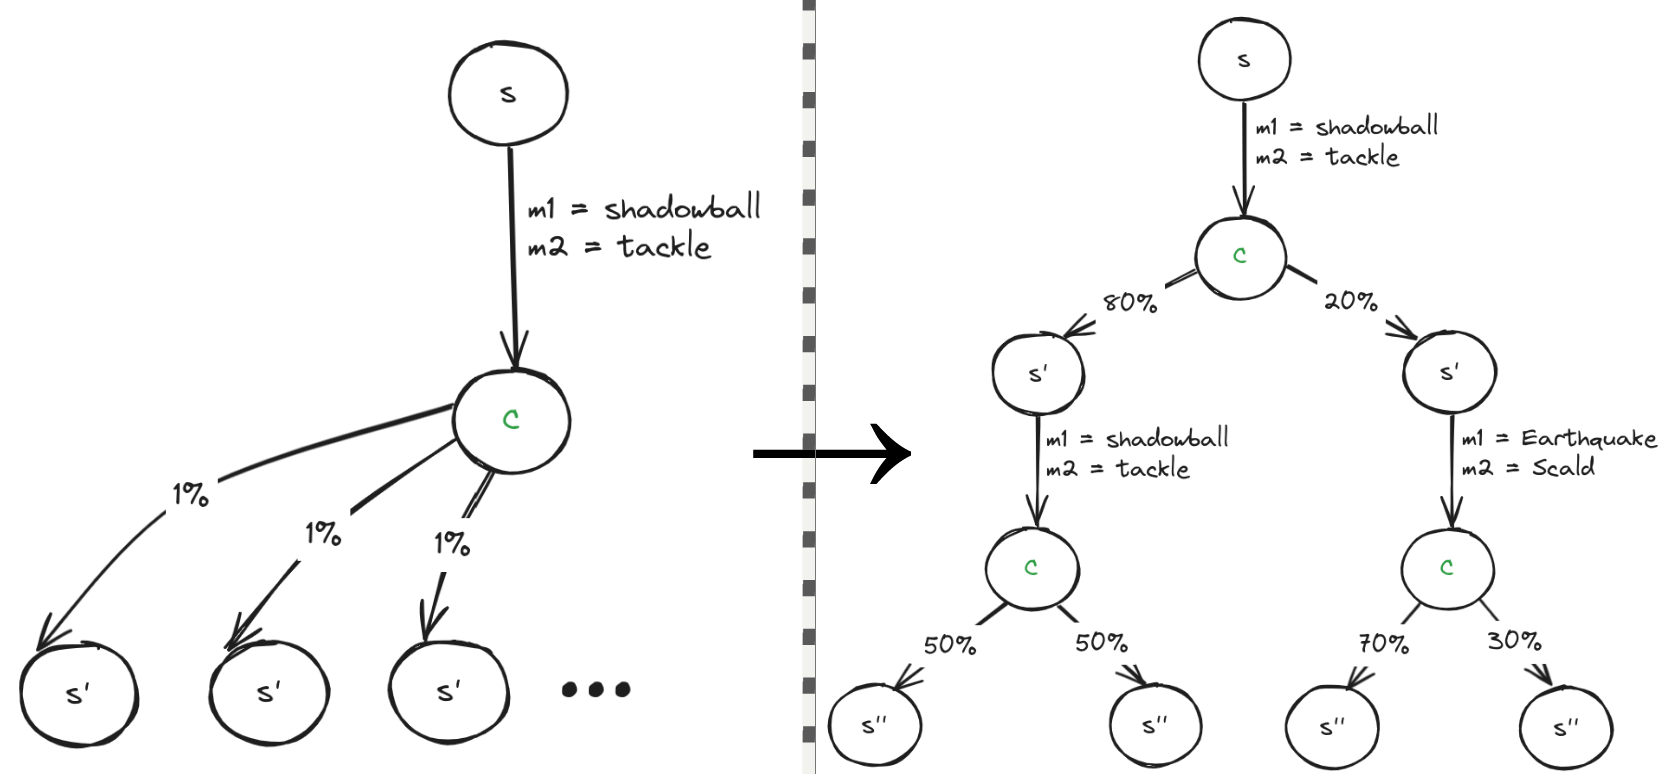
\includegraphics[width=0.8\textwidth]{figures/foulplay_search.png}
    \caption{Foul Play's MCTS search architecture with damage roll grouping. The engine clusters damage outcomes by knockout potential rather than exploring all 32 possible values (16 rolls $\times$ critical hit), enabling deeper search while preserving strategic relevance.}
    \label{fig:foulplay-search}
\end{figure}

\begin{figure}[h]
    \centering
    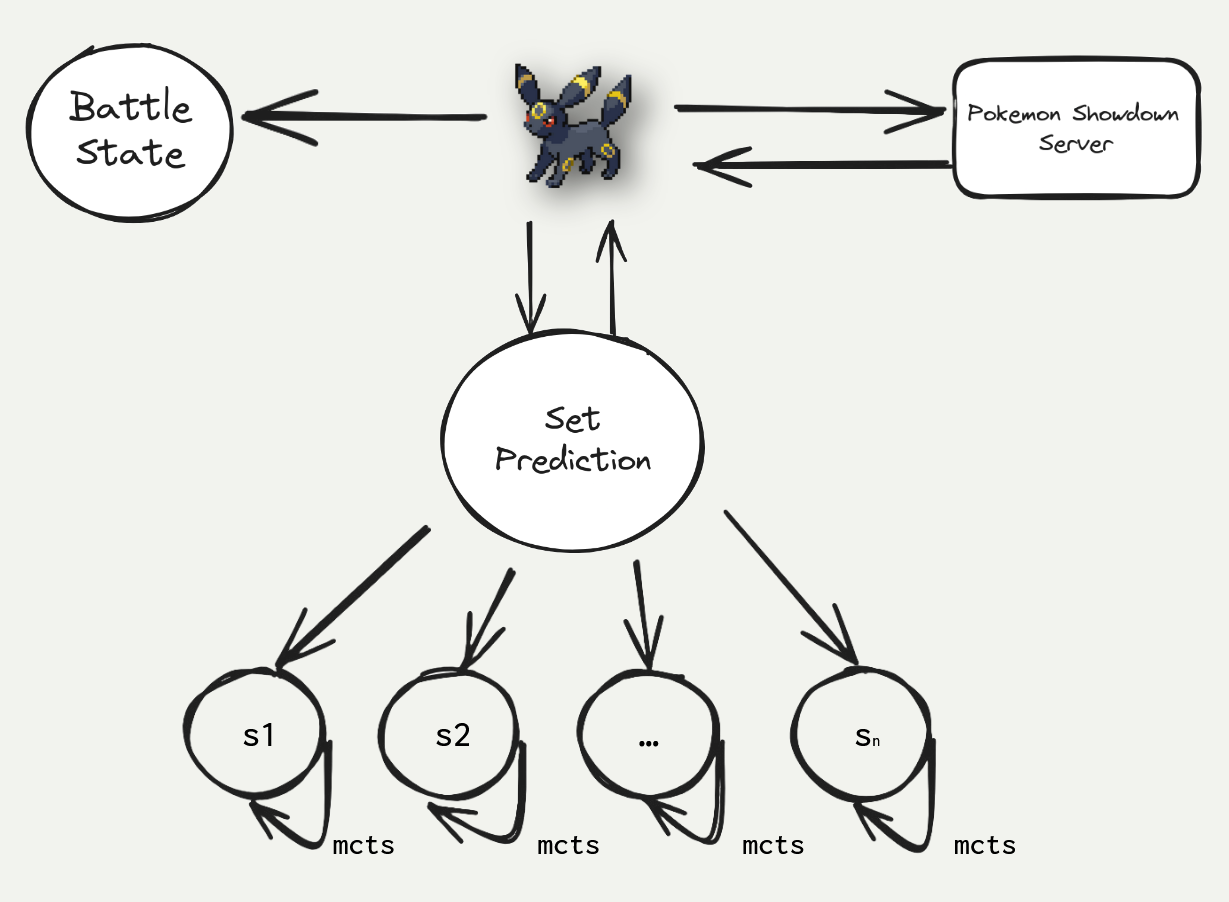
\includegraphics[width=0.6\textwidth]{figures/foulplay_prediction.png}
    \caption{Foul Play's set prediction pipeline. Hidden information is progressively inferred through damage calculations, priority ordering, weather duration, and move usage patterns, narrowing the space of possible opponent configurations.}
    \label{fig:foulplay-prediction}
\end{figure}

\subsubsection{4thLesson (Gen 1 OU Finalist)}
\label{sec:4thlesson}

\textbf{Team:} Gyungbo Kim, Sangyeon Park, Eunju Kwon, Yujin Kim \\
\textbf{Affiliation:} Pok\'eAgent Challenge Gen 1 OU Finalist

4thLesson follows Metamon's SyntheticRL-V2 model and adopts a fine-tuning approach starting from its pretrained model, while preserving the original architecture for stable initialization. Two key modifications distinguish their approach:

First, they employ the Kron (Kronecker-factored Approximate Curvature) optimizer instead of the AdamW optimizer originally used in the Amago framework. Although the Kron optimizer is a second-order optimizer and incurs higher computational cost than AdamW, recent work demonstrates that it stabilizes reinforcement learning by ensuring more consistent gradient flow when scaling up model size, outperforming Adam-based optimizers in this regard.

Second, they adopt AID (Activation by Interval-wise Dropout) instead of the previously used Leaky ReLU. AID introduces additional linearity into the model, mitigating plasticity loss in continual learning and reinforcement learning settings where model plasticity tends to degrade. Since AID also acts as a form of dropout, they removed the dropout modules used in the original model.

To collect high-quality self-play data, they employ a multi-stage data generation strategy based on a local ladder setup. They first generated self-play replays using the 19 baseline models provided by a local ladder setup, collecting approximately 30k replays for small-size models, 40k for medium-size models, and 50k--100k for large-size models. All replays were generated using the modern\_replays (v1) teamset, resulting in roughly 800k replays in total. In addition, they performed self-play between intermediate checkpoints of their own models, collecting another 300k--400k replays and increasing the total dataset size to approximately 1.1--1.2M replays. After the preliminary round, they repeated a similar process, generating about 10k samples per model, using the modern replays (v2) teamset and adding approximately 130k more samples, increasing the total dataset size to 1.3--1.4M samples.

\begin{figure}[h]
    \centering
    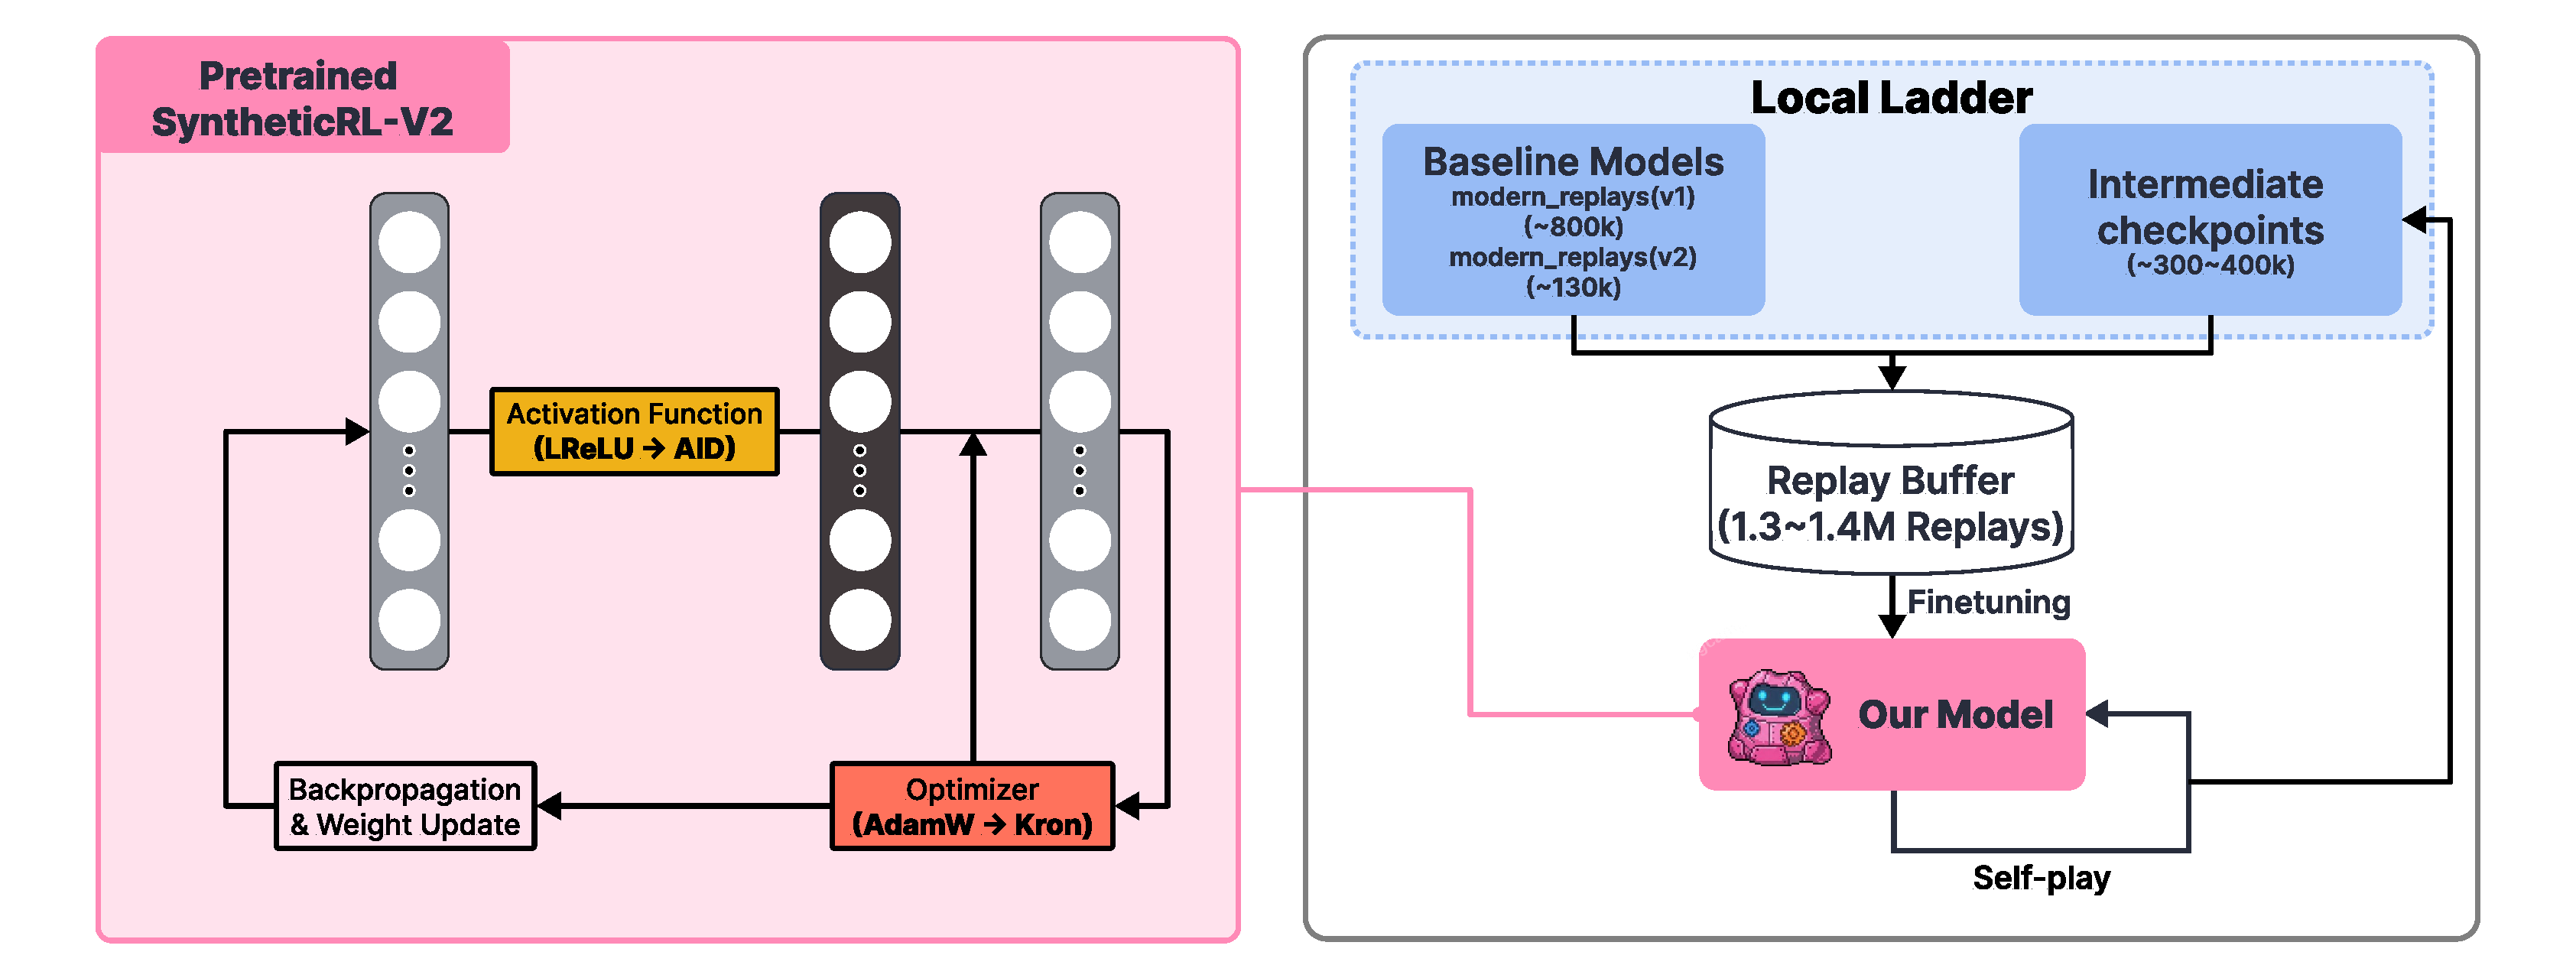
\includegraphics[width=0.9\textwidth]{figures/fourthlesson_method.pdf}
    \caption{4thLesson's learning architecture and training pipeline, showing the integration of the Kron optimizer and AID activation function.}
    \label{fig:4thlesson-method}
\end{figure}

\begin{figure}[h]
    \centering
    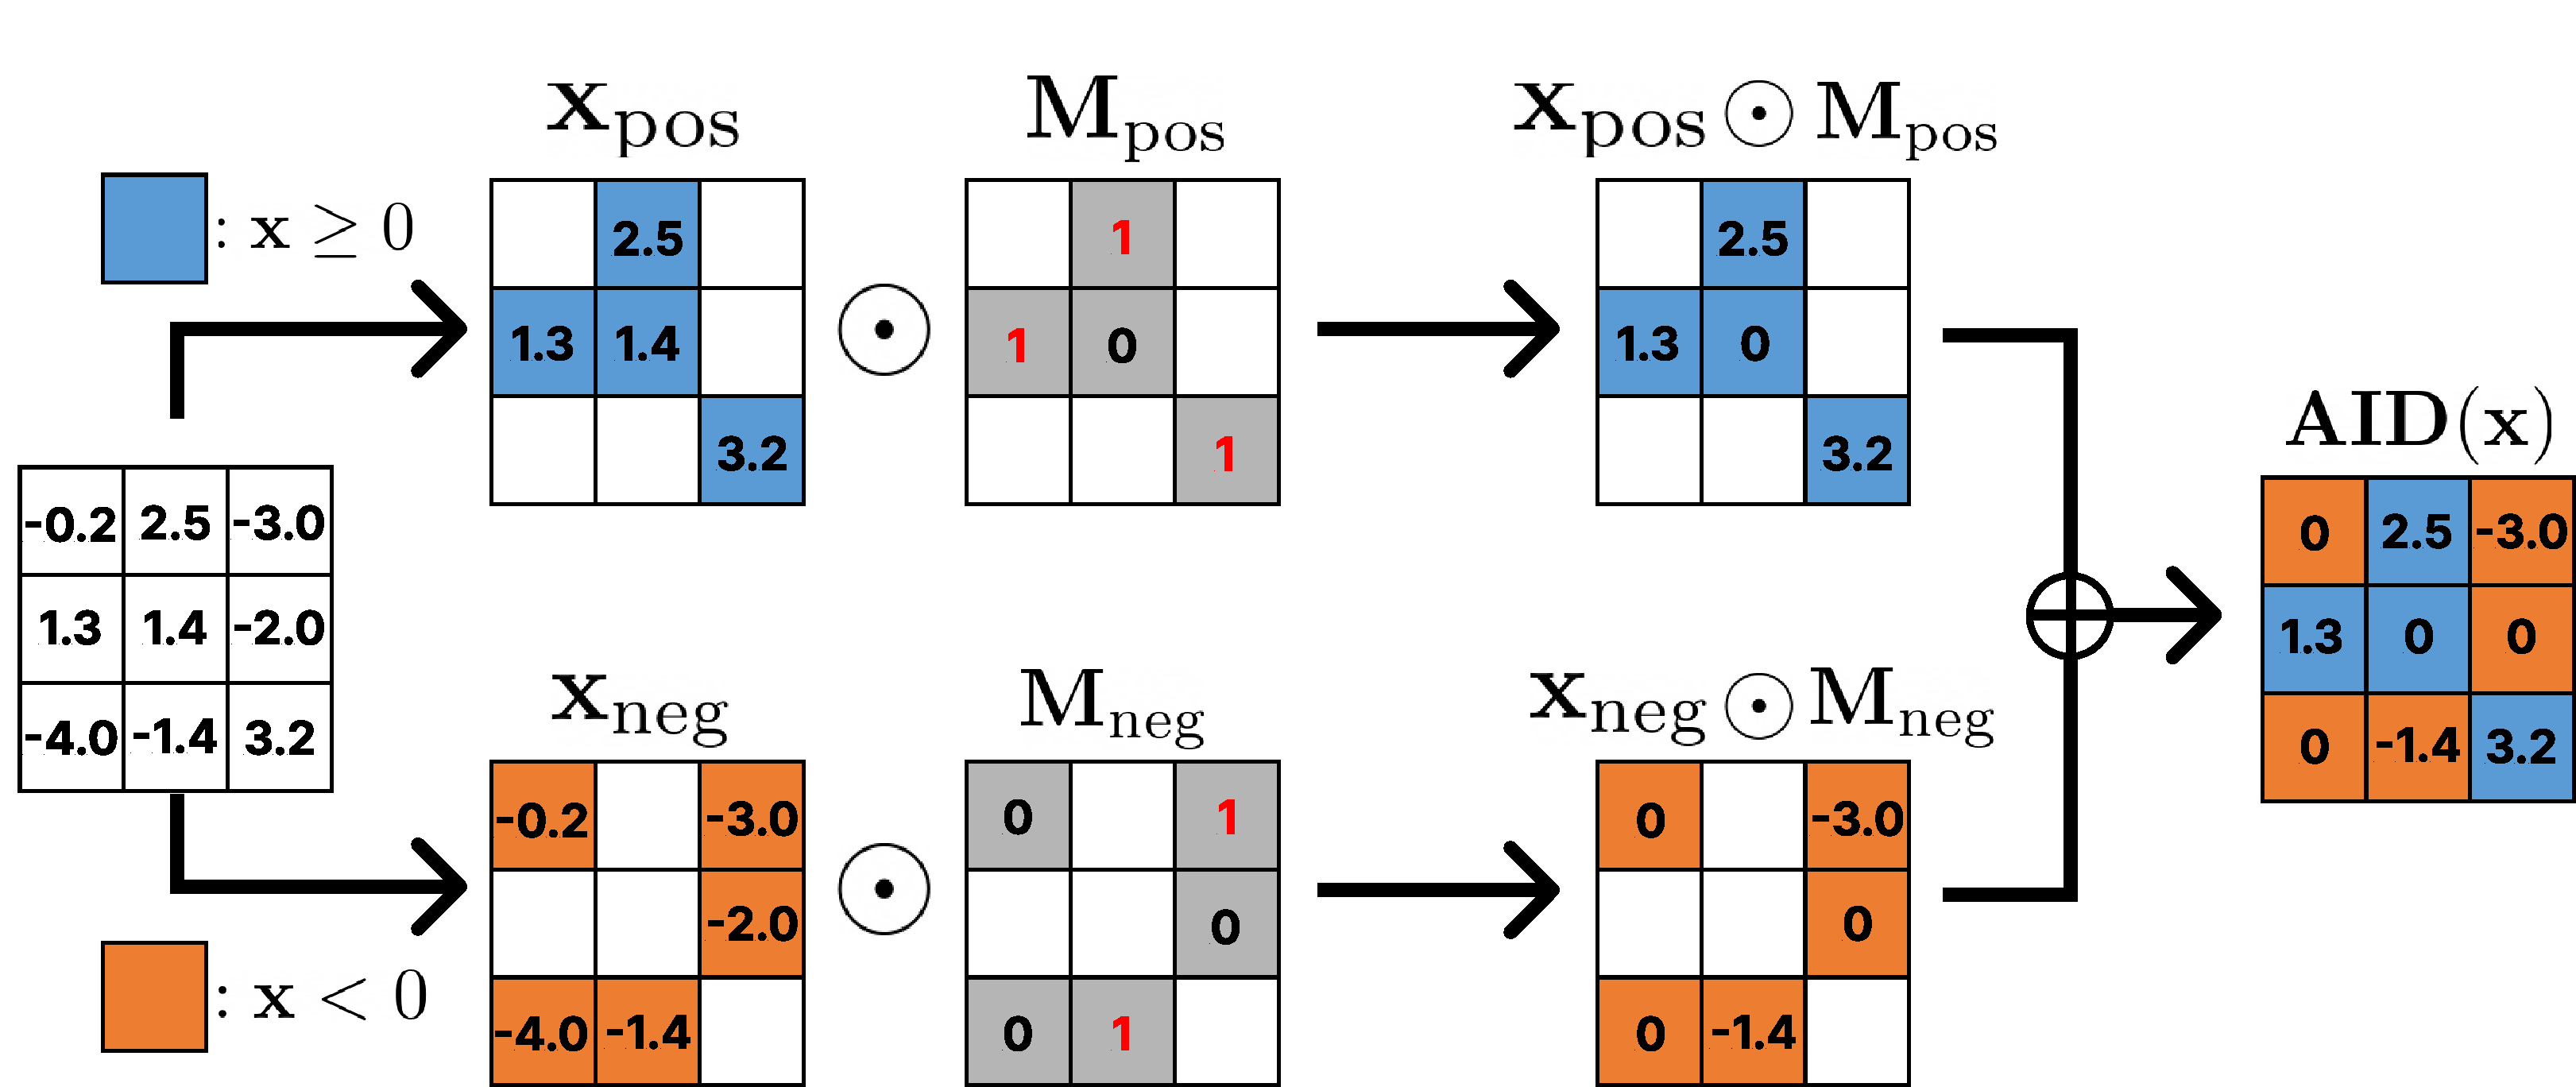
\includegraphics[width=0.6\textwidth]{figures/AID_method.pdf}
    \caption{Structure of Activation by Interval-wise Dropout (AID) used by 4thLesson to mitigate plasticity loss.}
    \label{fig:4thlesson-aid}
\end{figure}

\subsubsection{Team Q (Gen 9 OU Finalist)}
\label{sec:team-q}

\textbf{Team:} Qiao Wang, Ling Wu \\
\textbf{Affiliation:} Pok\'eAgent Challenge Gen 9 OU Finalist

Team Q's approach centers on a Two-Phase Curriculum Learning framework designed to bootstrap basic competency before refining advanced strategic reasoning. The agent architecture utilizes a 50M parameter Actor-Critic model. The core innovation lies in splitting the training process into two distinct phases: a \textit{Mechanics Phase} and a \textit{Strategy Phase}.

In the initial Mechanics Phase, the agent is fine-tuned against a suite of heuristic bots. This phase focuses on learning the fundamental rules of the game, such as type advantages, move effectiveness, and valid action masking, without the noise of complex adversarial behavior. Once the agent achieves a baseline win rate against these static policies, it transitions to the Strategy Phase. Here, they employ an iterative ``coach cycle'' where the agent trains against a fixed expert coach and previous versions of itself. This self-play and expert-play hybrid allows the agent to develop deeper foresight and prediction capabilities, resulting in a steady increase in win rates from version v0 to v6 as observed in their experiments.

Their results demonstrate that the separation of mechanics learning from strategic fine-tuning significantly accelerates convergence. The agent showed the most dramatic performance jumps when transitioning from the v0 team set (random/heuristic initialization) to the v1 team set (curriculum-based), validating the hypothesis that mastering low-level game dynamics is a prerequisite for high-level long-horizon planning in stochastic environments like Pokémon.

\begin{figure}[h]
    \centering
    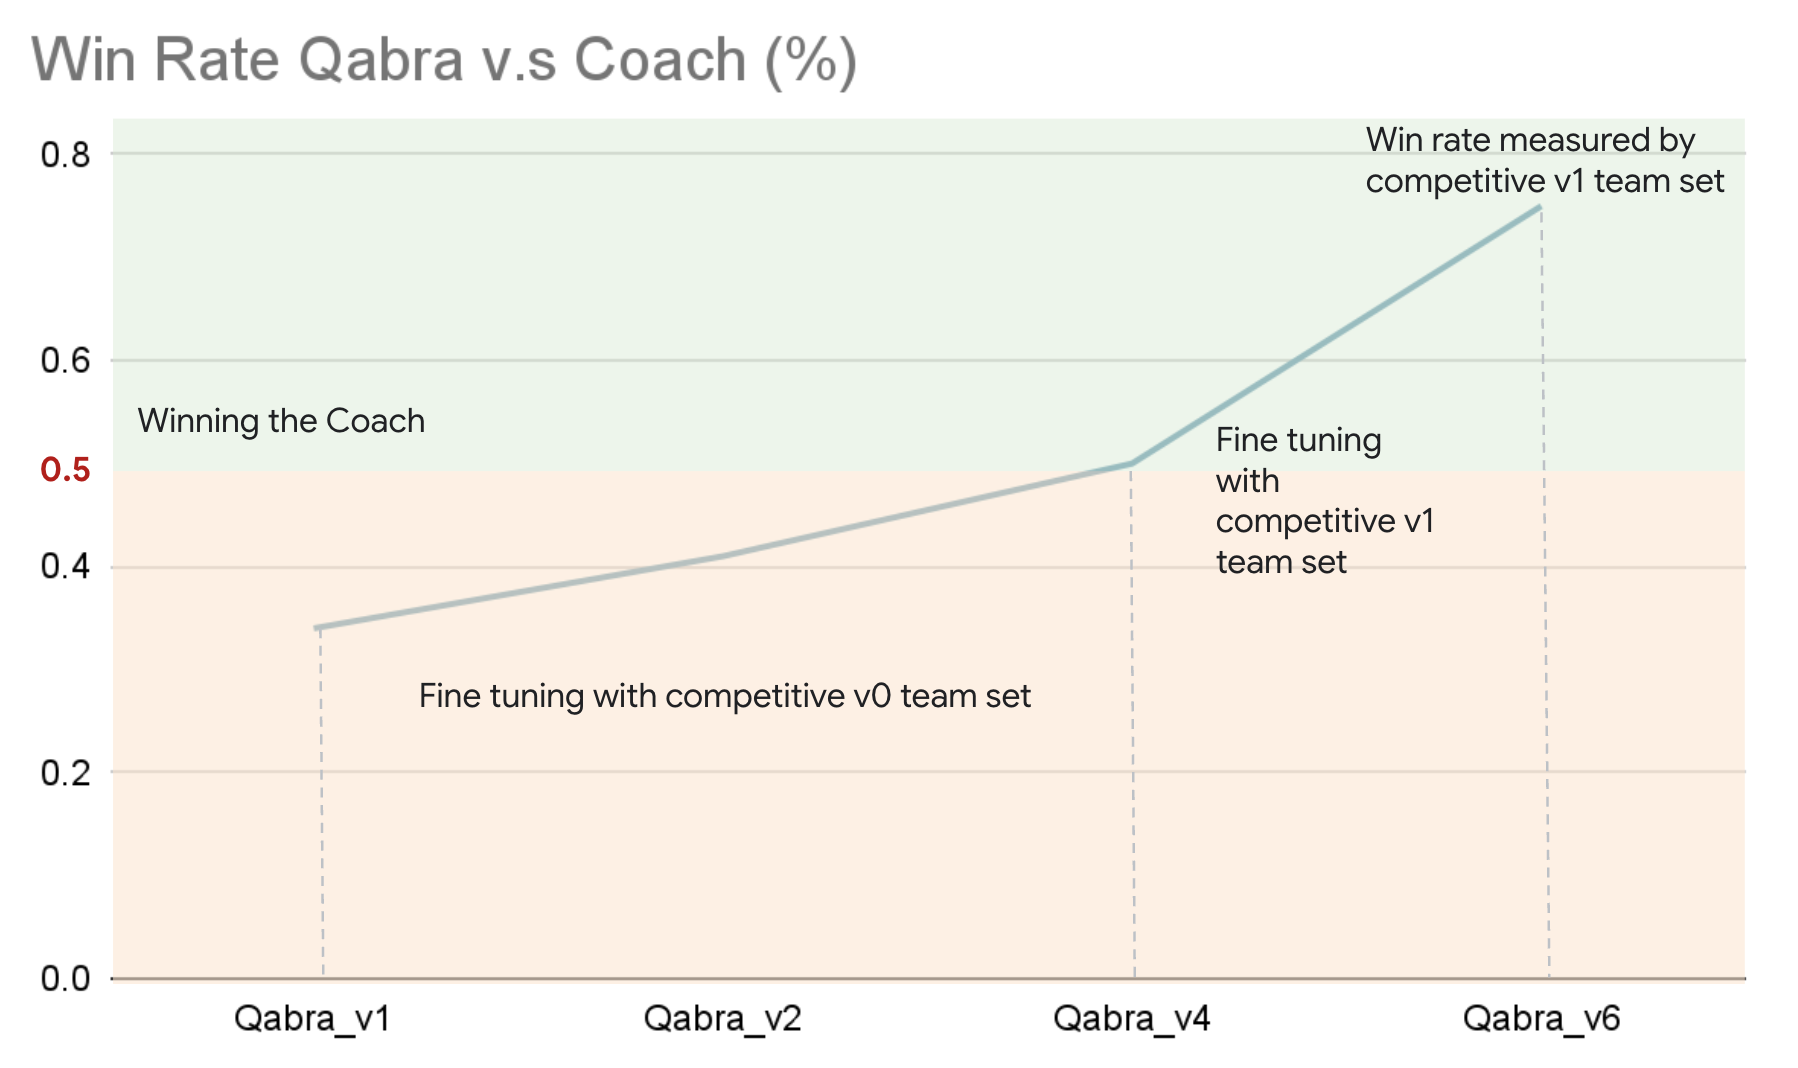
\includegraphics[width=0.65\textwidth]{figures/team_q_win_rate.png}
    \caption{Team Q's win rate performance across training iterations (v1--v6). Performance is measured against the Competitive v1 Team Set. The initial iterations (v1--v4) were trained on the v0 team set, while v6 incorporates fine-tuning on the v1 set, resulting in a performance jump to approximately 0.8.}
    \label{fig:team-q-winrate}
\end{figure}

\subsection{Speedrunning Track: RPG Speedrunning}

\subsubsection{Heatz (Speedrunning Track Champion)}
\label{sec:heatz}

\textbf{Author:} Junik Bae \\
\textbf{Affiliation:} Pok\'eAgent Challenge Speedrunning Track Champion

\begin{figure}[h]
  \centering
  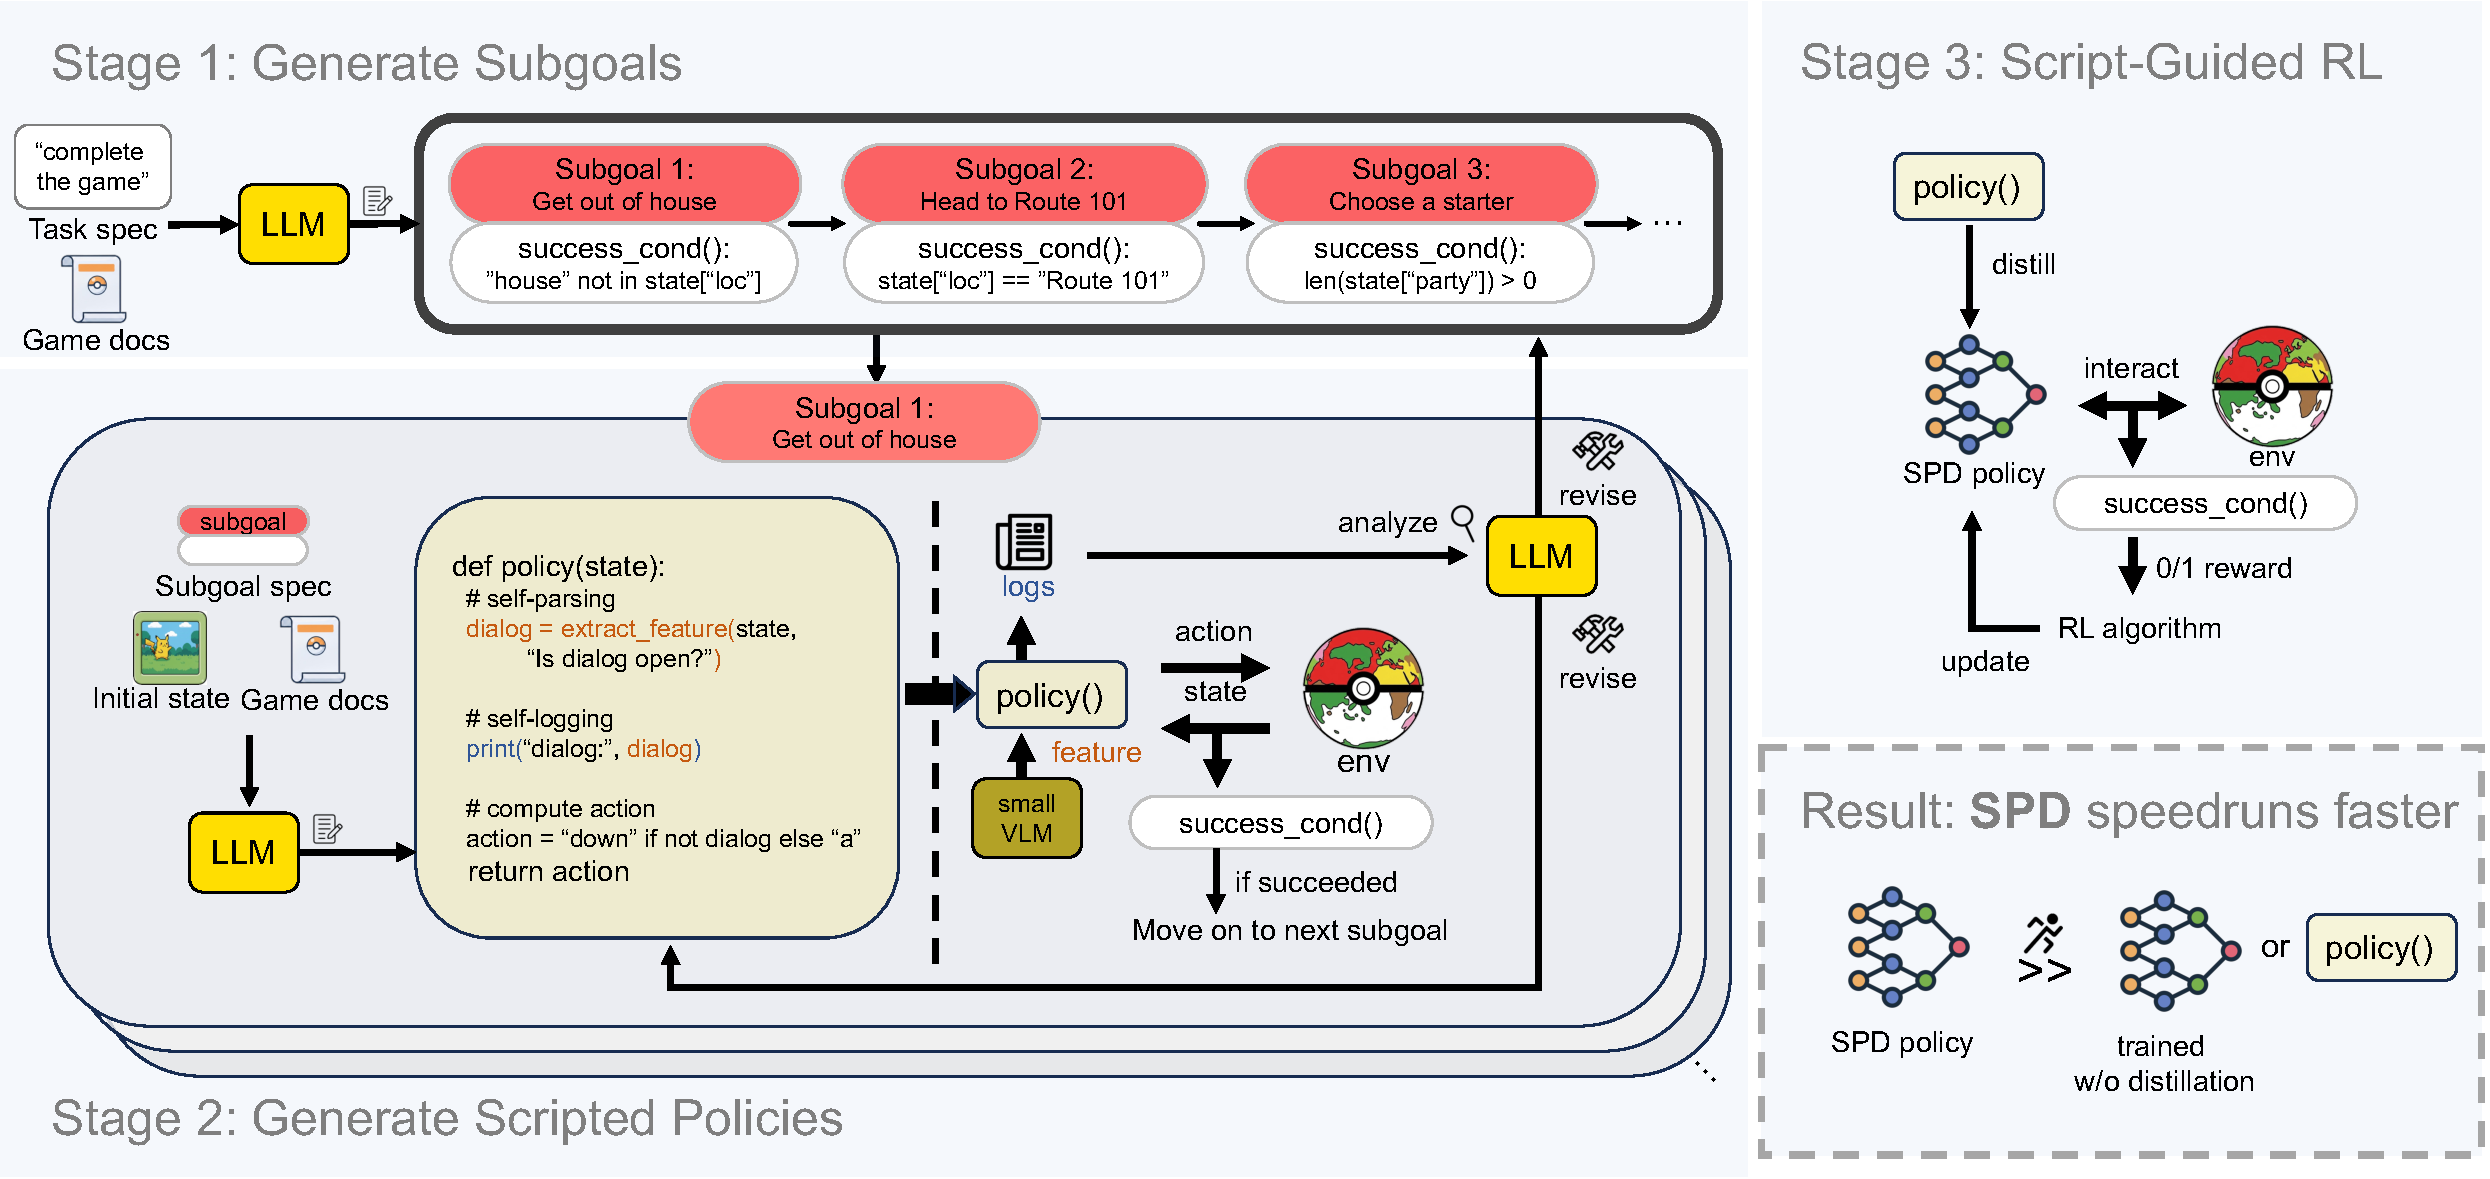
\includegraphics[width=\textwidth]{figures/heatz_figure.pdf}
  \caption{\textbf{Overview of Scripted Policy Distillation (SPD).} The approach consists of three stages: (1) Subgoal Generation where an LLM decomposes the task into sequential subgoals with executable success conditions; (2) Scripted Policy Generation where the LLM generates policies that can invoke VLM tools and use self-directed logging for debugging; (3) Script-Guided RL where scripted policies are distilled into neural networks via supervised learning followed by RL with expert action guidance.}
  \label{fig:heatz-method}
\end{figure}

Reinforcement learning (RL) offers a powerful framework for training autonomous agents, yet applying RL directly to long-horizon tasks with sparse rewards remains fundamentally challenging. To address this challenge, we propose leveraging LLM-generated scripted policies as priors for RL exploration (Figure~\ref{fig:heatz-method}). Although these scripted policies are not always optimal, they facilitate RL training by initializing exploration from a distribution that already reaches the goal, rather than from scratch. We implement this long-horizon task learning framework as \textbf{Scripted Policy Distillation (SPD)}, which consists of three stages: (1) subgoal generation~\citep{brohan2023can, zhu2023ghost}, (2) scripted policy generation~\citep{liang2023code, wangvoyager}, and (3) script-guided RL.

\paragraph{(1) Subgoal generation.} Given a long-horizon task specification, an LLM decomposes the task into a sequence of subgoals, each paired with an executable success-condition function \texttt{success\_cond(state)} that determines subgoal completion.

\paragraph{(2) Scripted policy generation.} For each subgoal, the LLM generates a \textit{scripted policy} that maps states to actions. The scripted policy interacts with the environment until \texttt{success\_cond(state)} returns \texttt{True} or a timeout occurs. Upon failure, the LLM analyzes execution traces and revises either the policy code (Stage 2) or the subgoal specification (Stage 1).

This stage employs two key techniques to handle complex environments. First, to extract rich visual cues that are not present in the state inputs, policies can optionally query a vision-language model (Qwen3-VL-8B) and use the resulting information for decision making. Second, to efficiently update subgoals and scripted policies, we provide the LLM with concise summaries of agent interactions obtained via \textit{self-directed logging}, rather than long, full execution trajectories.

\paragraph{(3) Script-guided RL.} Once all scripted policies reliably achieve their corresponding subgoals, we distill them into neural network policies via imitation learning on expert trajectories, followed by RL with expert action guidance. The resulting neural policies execute faster than the scripted policies and can therefore discover more efficient strategies.

For distillation, we train a DQN agent with two forms of expert guidance. First, we seed the replay buffer with successful expert trajectories. Second, during rollouts, we execute expert actions with probability $\epsilon$ (annealed from $0.1$ to $0$), while otherwise following the learned policy. Together, these mechanisms bootstrap learning from expert behavior while allowing improvements through RL optimization.

Our method, SPD, achieved a 40:13 run on Pokémon Emerald up to the first gym. The resulting policy exhibited several interesting emergent behaviors across the pipeline. During scripted policy generation, the agent occasionally synthesized explicit search routines, such as BFS over a local navigation graph, to reliably plan short paths for navigation subgoals. Furthermore, after distillation and RL fine-tuning, the neural policy executed these behaviors more efficiently and further improved speed through strategies not explicitly programmed in the scripts, including shorter routes, skipping unnecessary trainer battles, and faster menu interactions.

\subsubsection{Hamburg Pok\'eRunners (Speedrunning Track Second Place)}
\label{sec:hamburg}

\textbf{Team:} Benedikt Schink, Arian Urdu, Matin Urdu \\
\textbf{Affiliation:} Pok\'eAgent Challenge Speedrunning Track Second Place

Hamburg Pok\'eRunners achieved second place (first badge: 01:14:43) using a reinforcement learning approach based on recurrent proximal policy optimization (PPO). They used a standard recurrent PPO architecture with a long short-term memory (LSTM) in the recurrent state. The encoder consists of a convolutional neural network (CNN) and a multi-layer perceptron (MLP). The CNN receives downsampled game frames (grayscale, $128 \times 128$ pixels). A sinusoidal positional encoding is used to encode the $x$ and $y$ in-game coordinates. The location (e.g., the current city or route) is encoded using a one-hot encoding. Together, the location and the sinusoidal positional encoding result in unique positional coordinates. This global conditioning prevents the spatial ambiguity inherent in local coordinate systems.

The last input of the MLP is a binary milestone vector $m \in \{0, 1\}^{38}$, which encodes the sub-milestones of the competition, as well as the locations and Pok\'ecenters reached along the way. The milestone vector serves both as a memory component, keeping track of the milestones achieved thus far, and as goal-conditioning, keeping track of the current objective. This played a crucial role in making the model more stable to the inherent randomness of Pokémon Emerald and the non-deterministic input/output latency of the evaluation script. They observed simple error-correcting behavior, where the agent would overshoot or undershoot the target, resulting in backtracking to correct the trajectory.

Their reward function includes only positive rewards that incentivize desired behavior: competition sub-milestones, locations, coordinate exploration, badges received, money earned, HP healed, Pokémon leveled up, and damaging attacks used. All negative rewards they tried, such as step penalties, resulted in model degradation as the model reverted to only safe behavior and did not progress in the game.

Due to limited computational resources, they trained multiple smaller models that were then stitched together during inference, instead of training one larger model. Most attempts at transfer learning yielded only limited success, mostly helping with very basic navigation capabilities. While transfer learning yielded only small improvements restricted to basic navigation, the inclusion of a milestone vector significantly mitigated catastrophic forgetting.

\begin{figure}[h]
    \centering
    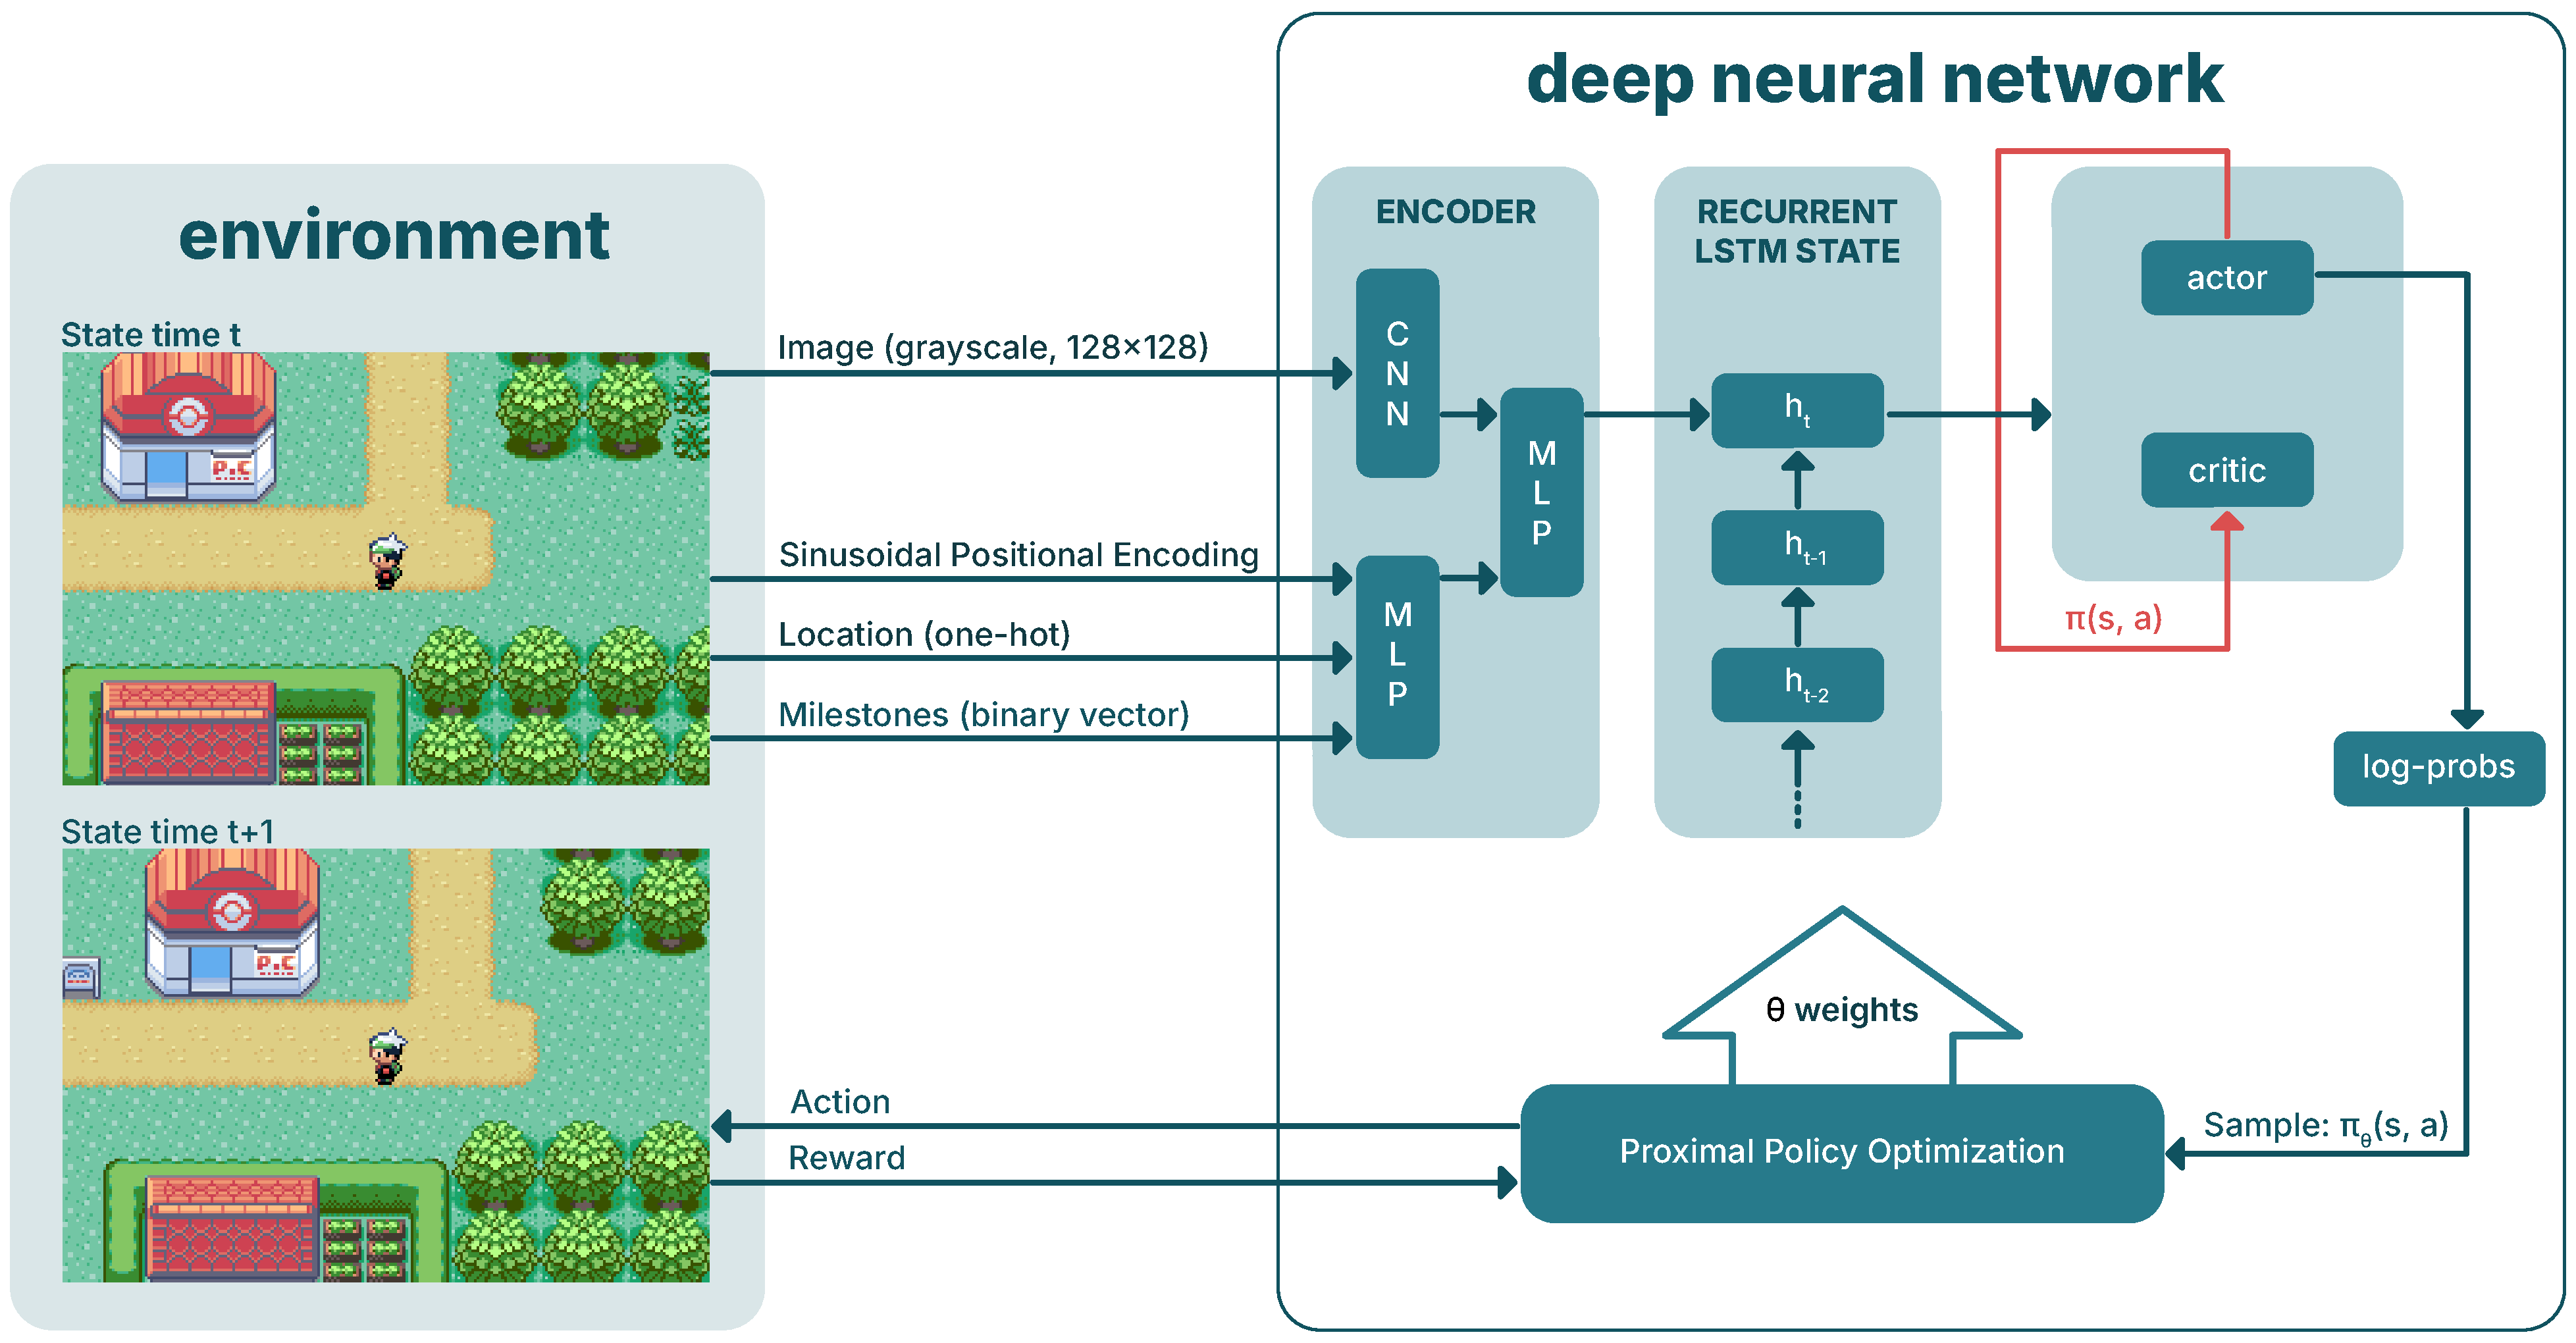
\includegraphics[width=0.8\textwidth]{figures/hamburg_architecture.pdf}
    \caption{Hamburg Pok\'eRunners' recurrent PPO architecture, showing the CNN encoder for visual input, MLP for positional and milestone encoding, and LSTM for temporal reasoning.}
    \label{fig:hamburg-architecture}
\end{figure}

\subsubsection{Anthonys (Speedrunning Track Third Place)}
\label{sec:anthonys}

\textbf{Author:} Anthony Sistilli \\
\textbf{Affiliation:} Pok\'eAgent Challenge Speedrunning Track Third Place

Anthonys' approach centered on decomposing the game progression into discrete phases with specialized navigation strategies for each context. The core innovation was combining deterministic pathfinding algorithms with context-aware prompt engineering to guide the language model through complex navigation and battle scenarios.

\textbf{Phase-Based State Management:} They structured the challenge into seven distinct phases, each corresponding to major game milestones. Each phase maintained its own prompt template with conditional instructions that dynamically adapted based on completed objectives and current location.

\textbf{A* Pathfinding with Directional Priorities:} Rather than relying solely on the LLM for spatial reasoning, they implemented A* pathfinding on the game map grid to compute optimal movement sequences. The system extracted walkable tiles from game memory, constructed a navigable grid representation, and generated action sequences to reach target coordinates.

\textbf{Battle State Management:} Battle sequences required special handling due to the game's menu system complexity. They implemented an input-clearing mechanism that sent predetermined button sequences to ensure the agent escaped bad states.

\textbf{Adaptive Recovery and Stuck Detection:} The system tracked position history to detect when the agent remained stationary for multiple turns, indicating an obstacle or navigation failure.

\subsubsection{Deepest (Speedrunning Track Judge's Choice: Most Efficient)}
\label{sec:deepest}

\textbf{Team:} Seonghun Hong, Hyunyoung Jeong, Hyeokgi Kim, Jaeyoon Jung \\
\textbf{Affiliation:} Seoul National University, Soongsil University, MAUM.AI

\begin{figure}[h]
    \centering
    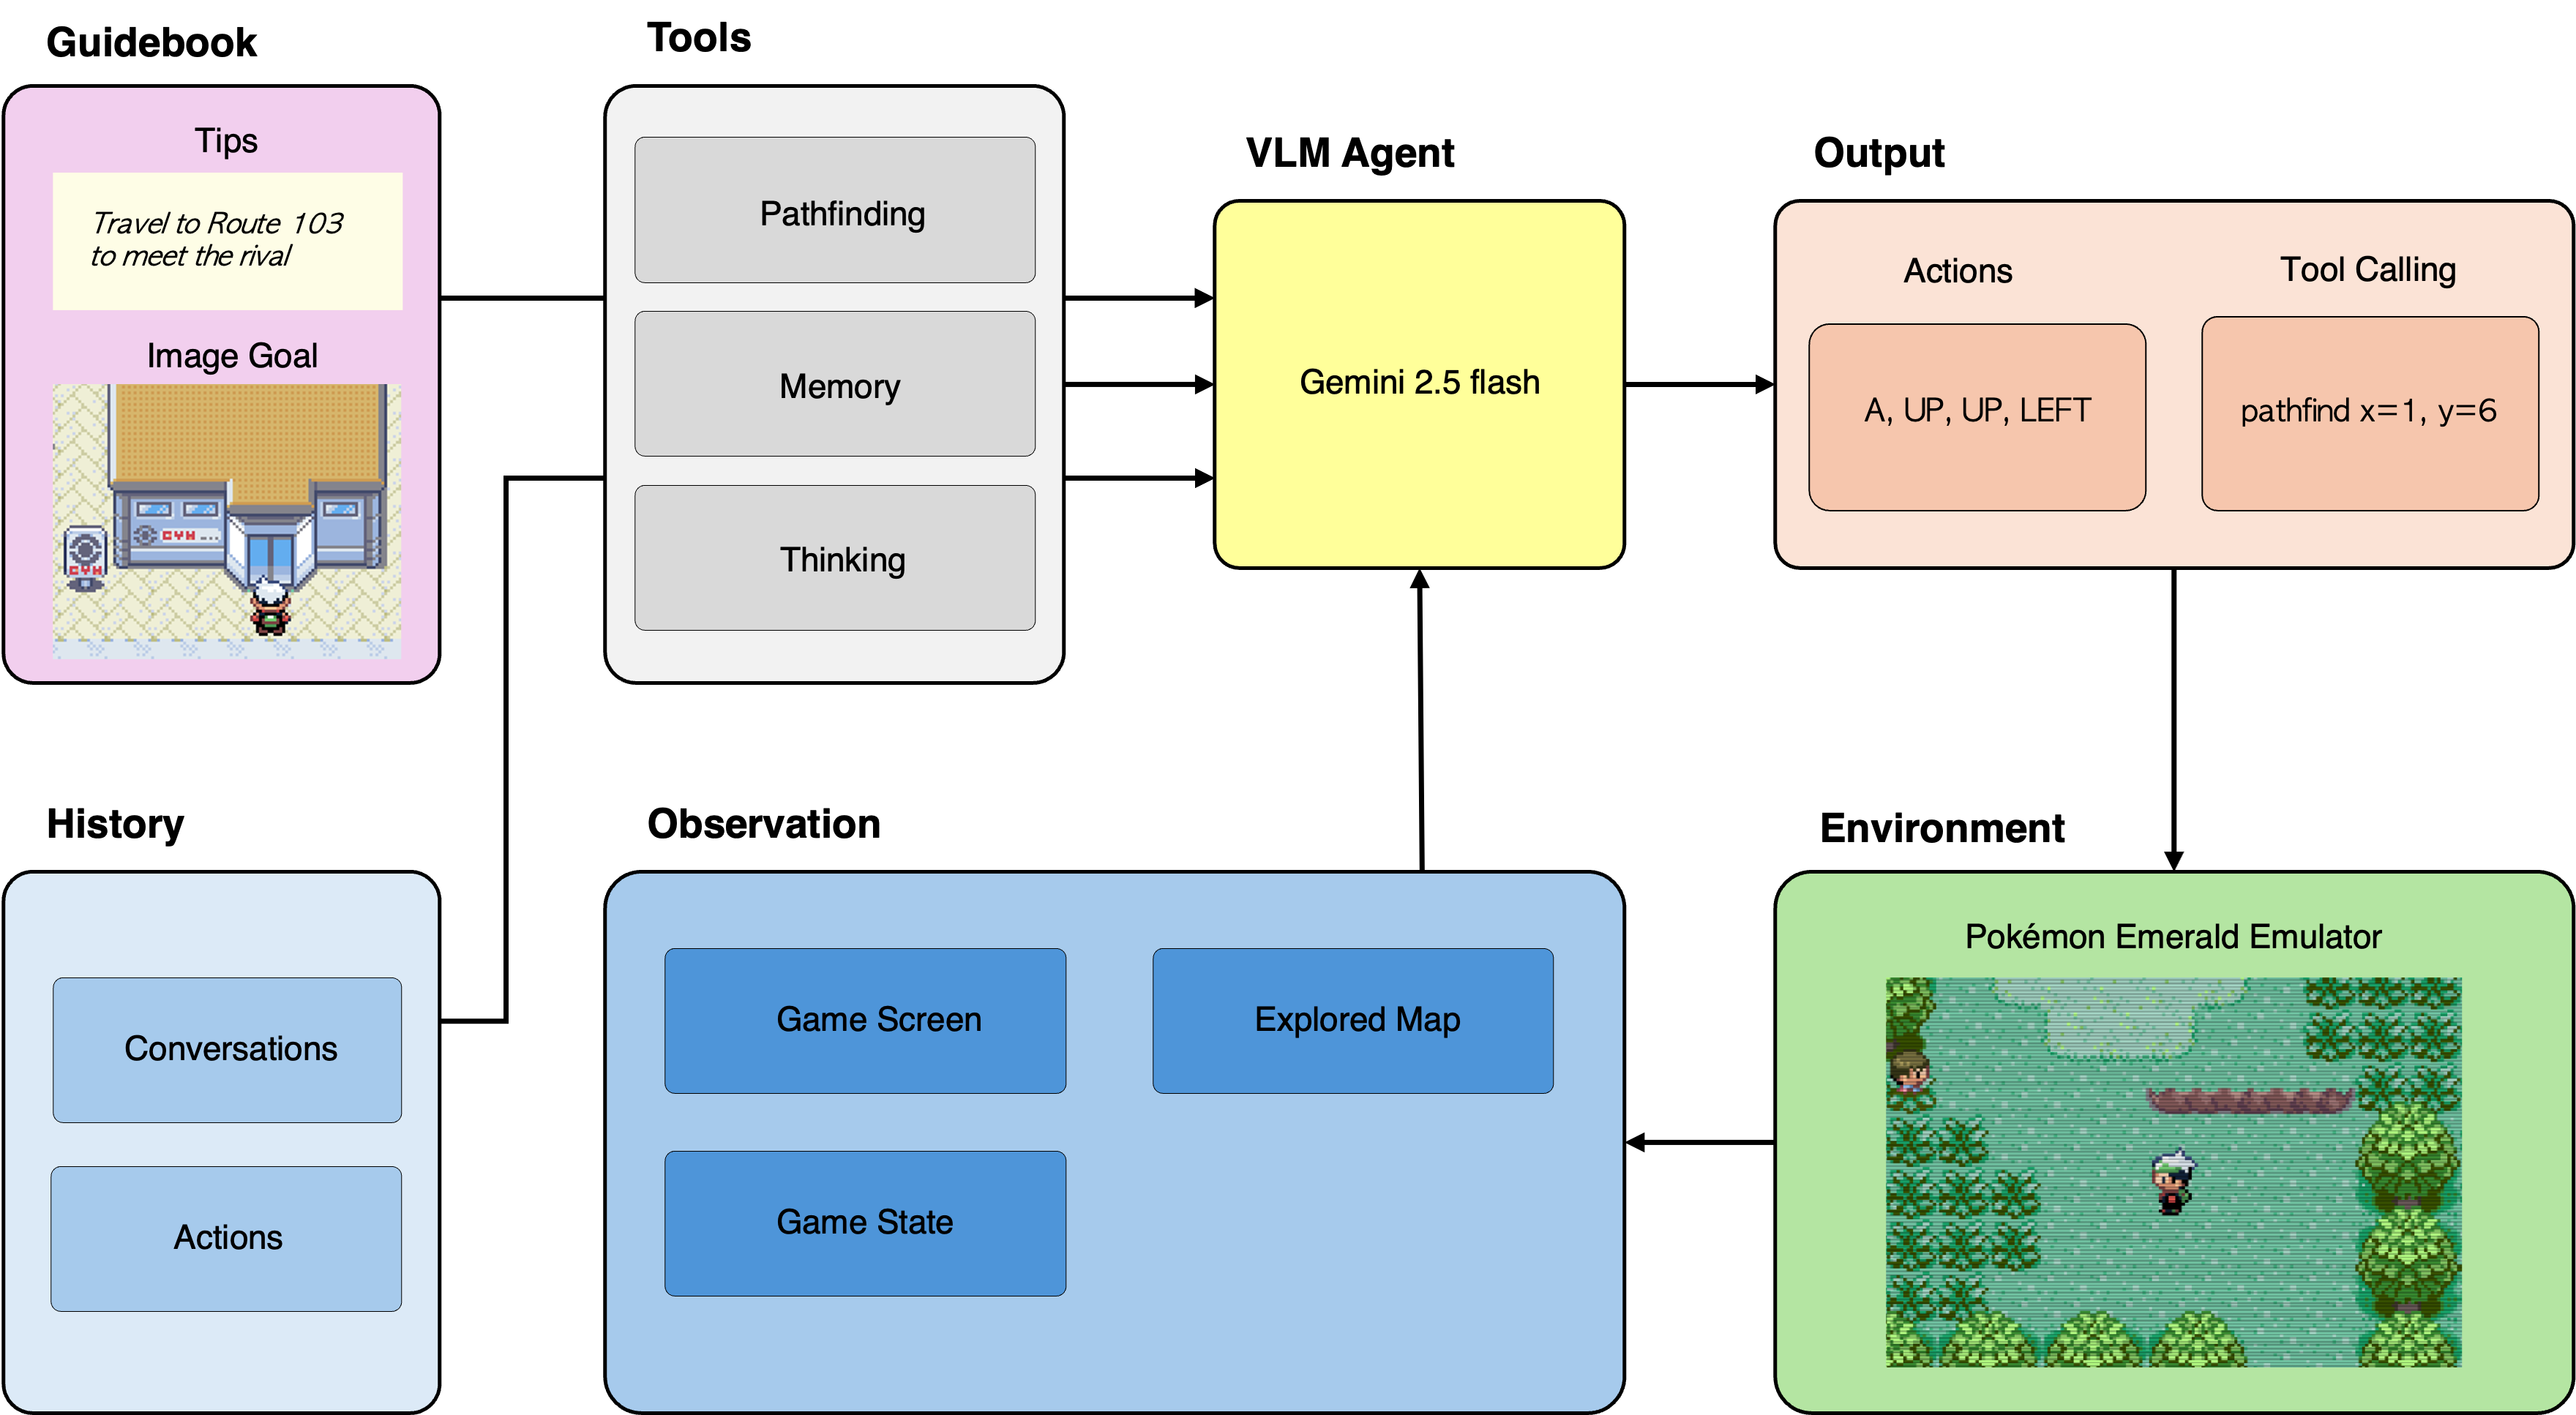
\includegraphics[width=0.92\textwidth]{figures/deepest_architecture.png}
    \caption{Deepest agent architecture overview. The agent receives partial observations and milestone-specific guidance from the Guidebook. Gemini 2.5 Flash reasons and outputs actions, optionally invoking tools (Pathfinding, Memory, Thinking). Actions execute in the emulator, producing the next observation. History provides temporal context.}
    \label{fig:deepest-architecture}
\end{figure}

We propose a training-free, fully autonomous agent architecture for Pokémon Emerald speedrunning that operates under human-like perceptual constraints using the Gemini 2.5 Flash vision-language model. Our approach achieved 5th place with a completion time of 02:04:29 for the first gym milestone and received the \textbf{Judge's Award} for most sample-efficient completion, demonstrating the effectiveness of principled agent design without data collection or human feedback.

A core design principle of our system is the absence of privileged game state. The agent receives no ground-truth map information; all navigation decisions---including those made by our pathfinding module---are computed exclusively from partially observed tiles explored during gameplay. This constraint closely mirrors human visual perception and ensures that planning and control emerge from observation-driven reasoning rather than access to internal game mechanics. To support high-level strategic decision-making, we introduce a \textbf{Guidebook} system inspired by how human speedrunners consult established guides. The guidebook provides milestone-specific knowledge, such as traveling to Route 103 to meet the rival and selecting Mudkip for type advantage against the Rock-type gym leader. For goal specification, we employ \textbf{image goals}---reference images of destination locations such as Professor Birch's Lab and Dad's Gym, which are visually indistinct buildings that are difficult to identify without prior game knowledge. These image goals enable the agent to visually recognize objectives and ground its actions in perceptual similarity. The overall architecture is illustrated in Figure~\ref{fig:deepest-architecture}.

Rather than relying solely on low-level action tokens (e.g., ``UP'', ``LEFT'', ``A''), we augment the agent with a set of auxiliary tools that allow it to autonomously reason, plan over long horizons, and adapt its computation, thereby better leveraging its decision-making capacity for efficient speedrunning. Specifically, we introduce three auxiliary tools:

\textbf{Pathfinding Tool:} This tool provides two navigation interfaces: coordinate-based navigation for known destinations, and directional exploration when exact coordinates are unknown. The pathfinder computes optimal trajectories on the observed map grid with the A* algorithm, incorporating game-specific constraints including one-way ledges and dynamic NPC collision avoidance.

\textbf{Memory Tool:} This tool supports long-horizon planning by enabling the agent to explicitly persist critical state information. To prevent the accumulation of stale or task-irrelevant information, we apply a sliding window policy that retains memory only over the most recent 10 conversation turns.

\textbf{Thinking Tool:} This tool implements adaptive computation by toggling the model's reasoning budget---allocating 2048 tokens for complex decisions while defaulting to 512 tokens for routine navigation.
